\documentclass[12pt]{article}

\usepackage{fontawesome}
\usepackage{hyperref}
\usepackage{xurl}
\usepackage{graphicx}
\usepackage{float}
\usepackage[tagged, highstructure]{accessibility}
\usepackage{bookmark}
\usepackage{enumitem}

\hypersetup{
    colorlinks=false,
    pdfborder={0 0 0},
    pdftitle={Reporting},
    pdfauthor={Adrianna Holden-Gouveia},
    pdfsubject={Advanced Data - Lab Assignment},
    pdflang={en-US},
    pdfkeywords={reporting, dashboards, North Star Metric, executive report}
}

% Configure PDF bookmarks for navigation
\bookmarksetup{
    numbered,
    open,
}

% Configure list spacing for better accessibility
\setlist{nosep}



\title{Reporting}
\author{
        Adrianna Holden-Gouveia \\
        Website: \href{https://aholdengouveia.name}{aholdengouveia.name}\\ 
        \date{\vspace{-5ex}}
        %Email: \href{mailto:admin@aholdengouveia.name}{admin@aholdengouveia.name} \\
%        \faLinkedin{: aholdengouveia} \\
        \faGithub {: aholdengouveia} \\
        %\faTwitter {: aholdengouveia} \\
        }

%S\date{\today}


\begin{document}    

\maketitle

%\begin{abstract}
%This is a template for Linux Administration Lab work
%\end{abstract}
%\tableofcontents


\section*{Accessibility Notice}
This document is also available in HTML format at:

Link: \href{https://aholdengouveia.name/AdvData/labs/wk14reporting.html}{\textbf{\nolinkurl{https://aholdengouveia.name/AdvData/labs/wk14reporting.html}}}

The HTML version provides enhanced accessibility features including keyboard navigation, screen reader support, responsive design, dark mode support, and high contrast options.

\section*{Request}
\noindent\textbf{Request:} DATA-7720\\
\textbf{Requested by:} Leadership team\\
\textbf{Data:} Your database, and your work from this term

\section*{Background}
It's the end of the term, and the leadership team wants to know what the data team found, and what to keep an eye on from now on. They want a one-page report they can act on, and a plan for a dashboard that shows the most important numbers at a glance.

\section*{Learning Outcomes}
By the end of this lab, you will be able to:
\begin{itemize}
    \item Evaluate dashboards for clarity and focus
    \item Choose a North Star Metric for a company, and measure it with SQL
    \item Decide whether a need calls for a report or a dashboard, and plan a dashboard
    \item Write an executive report with real numbers and a clear action item
\end{itemize}

\section*{Lab Instructions}
Use your own data set and company. Books are my example data only.

\subsection*{Screenshots}
Several parts of this lab ask for a screenshot. Each screenshot should have your name, term, and year.  One of the easiest ways to do that is make a text document with your name and term/year on your computer and save it to use all term. Any screenshots that don't include this information won't be counted.

\begin{figure}[H]
    \centerline{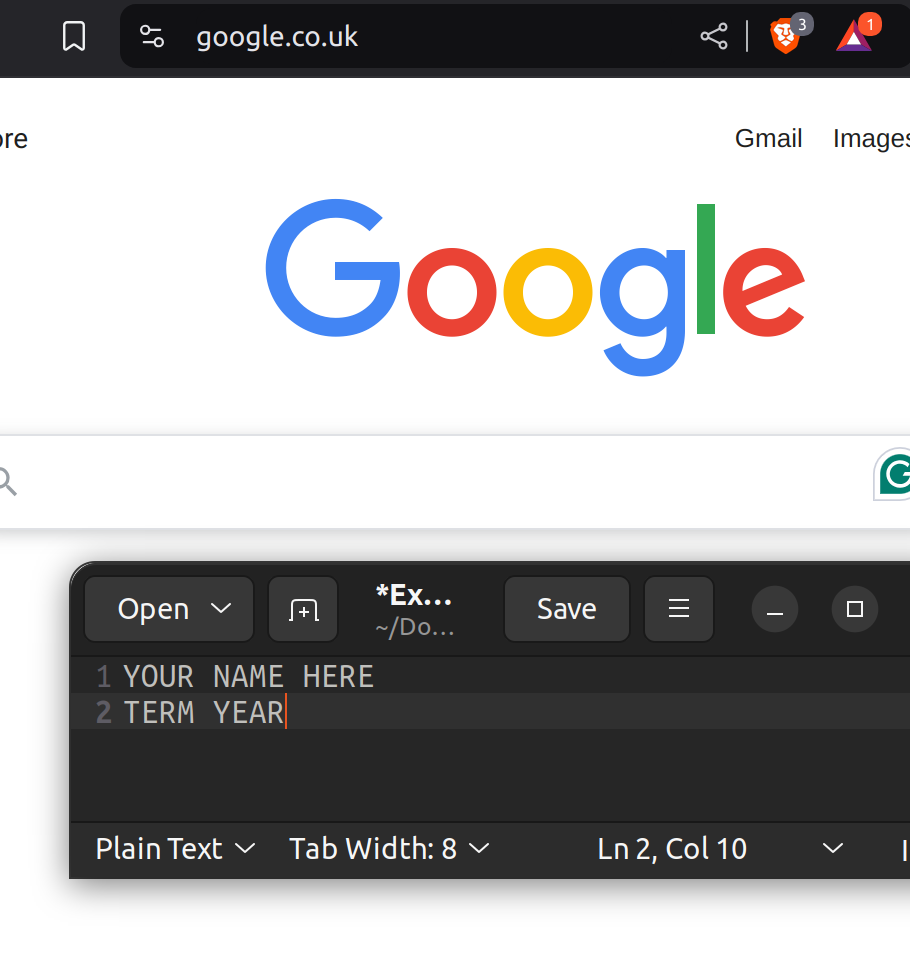
\includegraphics[scale=.2]{ExampleScreenshot.png}}
    \caption{This is an image of what each of your screenshots should look like}
    \alt{Example screenshot: a web browser showing the Google home page, with a small text editor window in front of it that says YOUR NAME HERE and TERM YEAR}
\end{figure}

\subsection*{Part 1: Good and Bad Dashboards}
Look at some real dashboards. I suggest Grafana Play, the live demo of Grafana, a free, open-source dashboard tool. It runs in your browser with no account, so you can click through real dashboards, change the time range, and see how often widgets refresh. The Tableau and Power BI dashboard examples are also good places to look. All are linked under Resources. Pick one example of a good dashboard and one of a bad dashboard, from any of these. In 1 or 2 paragraphs, compare them: what makes each one work or not work? Think about how clear it is, whether it focuses on key numbers, whether the charts suit the data, and whether it avoids common mistakes like clutter or information nobody needs. Include a screenshot of each one.

\subsection*{Part 2: Your North Star Metric}
\begin{enumerate}
    \item Pick a North Star Metric for your company: the one number that best shows whether it's succeeding. Explain why you chose it.
    \item Write and run a query on your database that measures it, and take a screenshot of the query and its results. If your database can't measure it yet, measure the closest thing you can, and explain what data you'd need to measure the real one.
\end{enumerate}

\subsection*{Part 3: Report or Dashboard?}
Pick 3 things someone at your company needs to know, such as daily sales, a summary for a compliance check, or whether the database is running out of space. For each one, decide whether it needs a report, a dashboard, or both, and explain why using the topic page.

\subsection*{Part 4: Dashboard Plan}
Plan a dashboard for your manager with 3 to 5 widgets, including your North Star Metric. For each widget, give:
\begin{enumerate}
    \item What it shows, and why your manager needs it
    \item The query it would use
    \item How often it should refresh, such as hourly, daily, or weekly, and why
\end{enumerate}
Then make a mock-up, also called a wireframe, of your dashboard, showing how the widgets would be laid out on one screen. Dashboards are usually planned this way before anyone builds them, so you don't need a dashboard tool or account. I suggest diagrams.net (linked under Resources), which you used in the Database Schema lab. It's free, runs in your browser with no account, and has mock-up shapes: select More Shapes at the bottom of the shapes list, and turn on Mockups. If you'd rather not use diagrams.net, you can:
\begin{itemize}
    \item Arrange your charts from the Data Visualization lab, and boxes for the other widgets, on one page of your document or on a slide
    \item Draw it on paper and include a photo, with your name and the term on the page
\end{itemize}
Label each widget so it matches your list, and include your name and the term on your mock-up.

\subsection*{Part 5: Executive Report}
Write a report of about one page for the leadership team, following the sample executive report (linked under Resources). Include:
\begin{enumerate}
    \item Its purpose, in a sentence or two
    \item At least 3 key findings from your queries, with real numbers
    \item One chart from the Data Visualization lab, with its alt text
    \item The data quality problems you found and fixed this term
    \item Your North Star Metric
    \item One clear action item for the leadership team
\end{enumerate}

\section*{Acceptance Criteria}
This request is done when:
\begin{itemize}
    \item Your dashboard comparison covers a good and a bad example, with a screenshot of each
    \item Your North Star Metric is explained, and measured with a query on your database
    \item All 3 needs have a report or dashboard decision, explained using the topic page
    \item Your dashboard plan has 3 to 5 widgets, each with what it shows, its query, and how often it refreshes, and a labelled mock-up
    \item Your executive report is about one page, uses real numbers from your queries, and ends with one clear action item
    \item Every screenshot follows the screenshot rules
\end{itemize}

\section*{Deliverables}
One file that includes Parts 1 to 5.

Audience: the leadership team, who aren't technical. Parts 1 to 4 can be technical, since the data team will check them.

\section*{Resources}
References, a video, a PowerPoint and some notes are available at my website
Link: \href{https://www.aholdengouveia.name/AdvData/Reporting.html}{\textbf{\nolinkurl{https://www.aholdengouveia.name/AdvData/Reporting.html}}}

Sample executive report, for Part 5
Link: \href{https://www.aholdengouveia.name/AdvData/labs/SampleExecutiveReport.txt}{\textbf{\nolinkurl{https://www.aholdengouveia.name/AdvData/labs/SampleExecutiveReport.txt}}}

Suggested: Grafana Play, live dashboards in your browser with no account
Link: \href{https://play.grafana.org/}{\textbf{\nolinkurl{https://play.grafana.org/}}}

Tableau dashboard examples
Link: \href{https://www.tableau.com/dashboard/dashboard-examples}{\textbf{\nolinkurl{https://www.tableau.com/dashboard/dashboard-examples}}}

Power BI sample reports and dashboards
Link: \href{https://learn.microsoft.com/en-us/power-bi/create-reports/sample-datasets}{\textbf{\nolinkurl{https://learn.microsoft.com/en-us/power-bi/create-reports/sample-datasets}}}

diagrams.net, for your dashboard mock-up
Link: \href{https://app.diagrams.net/}{\textbf{\nolinkurl{https://app.diagrams.net/}}}

My CSV to Database Converter, for turning query results into a CSV file
Link: \href{https://www.aholdengouveia.name/AdvData/labs/csv-to-database.html}{\textbf{\nolinkurl{https://www.aholdengouveia.name/AdvData/labs/csv-to-database.html}}}

\end{document}